\documentclass[12pt]{article}
\usepackage{hyperref}
\usepackage[utf8]{inputenc}
\usepackage[T1]{fontenc}
\usepackage{graphicx}
\hypersetup{colorlinks=true,linkcolor=blue, linktocpage}
\begin{document}
\section*{Risengrynsgr{\o}t, 03.01.2019}
\begin{itemize}
\item Oppskrift:
  \begin{itemize}
  \item Pr{\o}vde {\aa} sette gr{\o}ten i ovnen, men en time etterp{\aa} hadde
    ingenting skjedd s{\aa} gikk tilbake til f{\o}lgende
    \href{https://www.melk.no/Oppskrifter/Groeter/Tradisjonsgroet/Risengrynsgroet}{oppskrift}
    med 3~dl seterr{\o}mme.
  \end{itemize}
\item Kommentarer:
  \begin{itemize}
    \item Tok veldig lang tid (ca tre timer), vil nok kj{\o}re p{\aa} med
      h{\o}yere varme neste gang fra start og r{\o}re ofte. Satt seg ikke
      s{\ae}rlig fast i bunnen (overraskende).
  \end{itemize}
\item Konklusjon:
  \begin{itemize}
  \item Smakte helt ok, kanskje litt vassent, men vet ikke helt hvordan dette kan forbedres (lavere varme?). 
  \end{itemize}
\end{itemize}
\centering
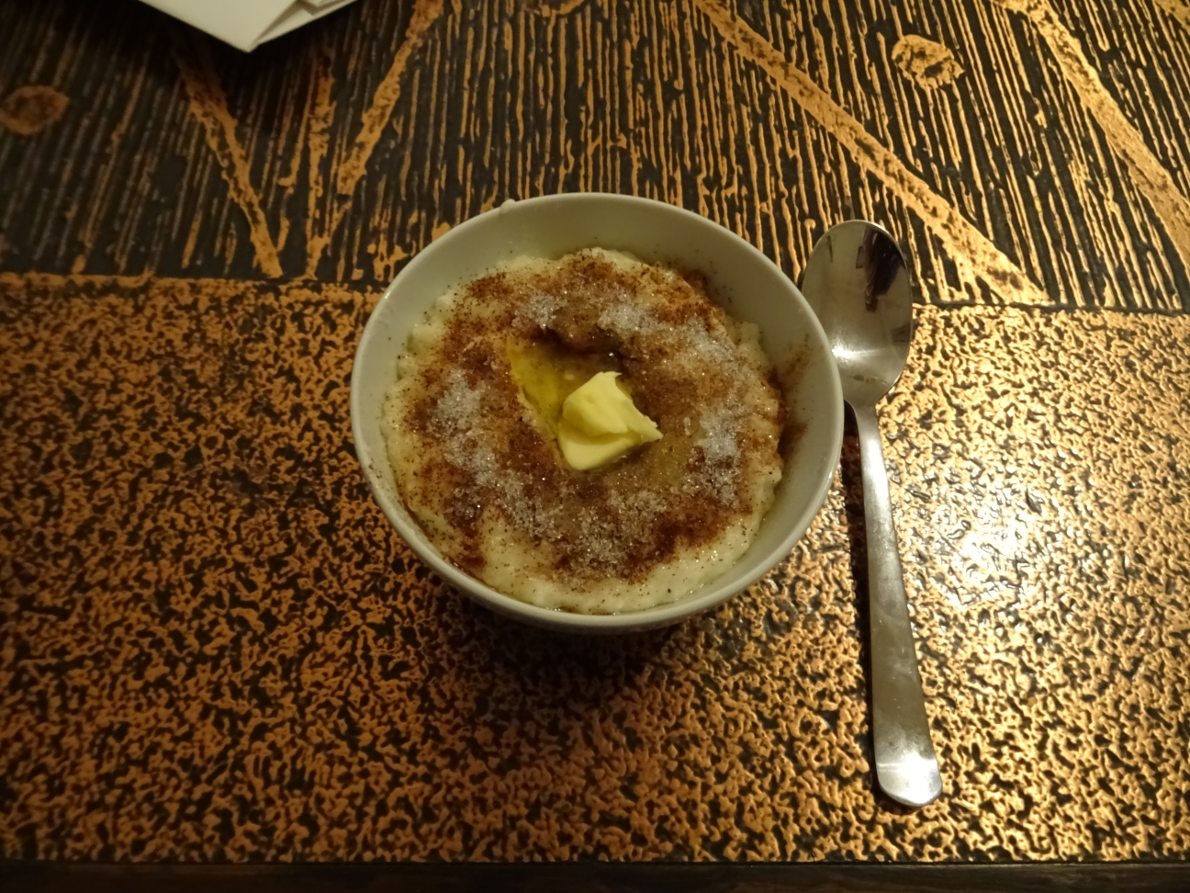
\includegraphics[width=3.33in]{03-01-2019.png}
\end{document}

